\documentclass[12pt,info]{asg}
% General info for the asg.cls file to load
\Instructor{Anna Koop}
\Campus{University of Alberta, Augustana}
\Email{akoop@ualberta.ca}
\Office{Heather Brae 1-31}
\Class{AUCSC 370}
\ClassTitle{Programming Languages}
\Term{Fall 2016}
\Department{Department of Science}


\AsgNum{2}
\AsgTitle{Scheme Intro Assignment}
\Due{11:55pm, Oct 13, 2016}
\Total{3}

\title{Feature Vector Representation}

\begin{document}

\maketitle
\section*{Objectives}
\begin{itemize}
\item To become familiar with Scheme syntax and semantics.
\item To learn how to use Scheme lists to represent data.
\item To become familiar with Scheme's list-handling primitives.
\item To become acquainted with the techniques of pure functional programming.
\item To gain fluency in thinking and programming recursively.
\end{itemize}

Adapted from the Polynomial assignment from Jonathan Mohr.

\section*{Specification}
Write a set of scheme functions for manipulating feature vectors of the form:
\begin{equation}
[x_0, x_1, ... x_n].
\end{equation}

\paragraph{makeVector} Given a list of integers, returns feature vector. The integers are guaranteed to be in the form:
\begin{equation}
(<index><value><index><value>....)
\end{equation}
subject to the following constraints:
\begin{itemize}
\item The indices are in strictly ascending order from left to right (i.e. none are equal).
\item No value is zero except for the last index (which may used to indicate the maximum size of the vector).
\end{itemize}

For example, the input:
\begin{equation}
(0\ 1\  1\  4\  3\   {-2}\ 10\  65\  11\  0)
\end{equation}
would represent the features:
\begin{align*}
x_0 & = 1\\
x_1 & = 4\\
x_3 & = {-2}\\
x_{10} & = 65\\
x_{11} &= 0
\end{align*}
or in vector notation:
\begin{equation}
[1, 4, 0, {-2}, 0, 0, 0, 0, 0, 0, 65, 0]
\end{equation} 

It is up to you to decide how you want to represent the features internally. If you decide that the format of the input is the best representation, then \texttt{makeVector} will simply return the input. If you want to represent it explicitly as a list of pairs, then, given the previous sample input, your function should return:
\begin{equation}
((0\  1)\  (1\  4)\  (3\  {-2})\  (10\  65)\  (11\  0)).
\end{equation}
Or you may wish to store as a flat list echoing the vector notation, in which case your function should return:
\begin{equation}
(1\  4\  0\  {-2}\  0\  0\  0\  0\  0\  0\  65\  0).
\end{equation}

You may write the following functions assuming that their arguments are formatted according to the output of your \texttt{makeVector} function. For example, I might test your \texttt{addVector} and \texttt{writeVector} functions (see below) as follows:
\begin{lstlisting}[language=Lisp]
(writeVector (addVector (makeVector (read)) (makeVector (read))))
\end{lstlisting}

More likely, I would use a test function which defines two vectors and tests your \texttt{addVector} and \texttt{writeVector} functions as follows:
\begin{lstlisting}[language=Lisp]
(define v1 '(0 3 1 4 2 5))
(define v2 '(1 5 3 -1 10 0))
(writeVector (addVector (makeVector p1) (makeVector p2)))
\end{lstlisting}

\paragraph{writeVector} accepts a vector argument and prints a representation of it in the form:
\begin{equation}
[x_0, x_1, x_2, .... x_n]
\end{equation}
where the $x_i$ values are replaced with 0 or the vector values as appropriate (see vector notation above).

\paragraph{writePrettyVector} accepts a vector argument and prints a representation of it in the form:
\begin{align*}
\text{x0} & = x_0\\
\text{x1} & = x_1\\
\cdots\\
\text{x}n & = x_n
\end{align*}
where only the non-zero and final values are printed, $x_i$ values are replaced with the appropriate vector values, and $n$ is the largest index in the vector (see example above).

\paragraph{addVectors} accepts two vector arguments and returns a vector which is their sum.

\paragraph{subVectors} accepts two vector arguments and returns a vector which is the first minus the second.

\paragraph{dotProdVectors} accepts two vector arguments and returns a vector which is the length of the longest, where each element is the product of the corresponding elements in the input vectors.

\paragraph{meanVector} accepts a single vector argument and returns the mean value of the elements. Note that this must take the full length of the vector into account.

\paragraph{maxVector} accepts a single vector argument and returns the maximum value within the vector.

\paragraph{argmaxVector} accepts a single vector argument and returns the {\em index} 
of the maximum value within the vector. 

\section*{Details}
Your implementation is subject to the constraint that it should illustrate pure functional programming: that is, it should not use \texttt{define} to assign an object to a variable (only to define functions), nor use \texttt{set!} or its variants. You may use \texttt{define} for the purposes of testing your other functions, as illustrated above, but not within any of the assigned functions. 

You may, of course, define any other subsidiary functions which you might find useful. For example, a function which calculates the sum of the vector might come in handy for calculating the mean.

\paragraph{WARNING}: Make sure you define your functions as described! For example, functions that take multiple arguments end with an \texttt{s} and functions that take a single argument do not. If the functions are not structured according to the specification they will not be marked!

Submit the source code for your solution using eClass.

\section*{Grading}
Your solution should display the following characteristics:
\subsubsection*{Correctness, 40\%}
The program should conform to the specifications for which it was written. It should include correct handling of special cases, error conditions, etc.
\subsubsection*{Design and Efficiency 25\%} The program should be constructed from small, coherent, independent and loosely coupled functions. Each function should access only its own local variables and parameters and, in some cases, global constants. The control constructs and data structures used should be those appropriate to the problem at hand. The program should not perform unnecessary steps, use extraneous variables, nor implement the algorithm in a contorted or inefficient way.
\subsubsection*{Style and Documentation 25\%} The program should conform to generally accepted principles of style, such as a consistent pattern of indentation, use of meaningful identifiers and defined constants, generous use of space, etc. Internal documentation should include program and function headers, and in-line comments to clarify the code.
\subsubsection*{Knowledge of the language 10\%} Your program should provide evidence of your familiarity with the principal control constructs, operators, built-in functions, and data structuring facilities of the assigned language. 

In the case of Scheme, you should also demonstrate your grasp of the principles of functional programming. Comments should be prefixed according to the standard practice in Scheme.
%%%%%%%%%%%%
%\begin{figure}[bt]
%\label{fig:adder}
%\centering
%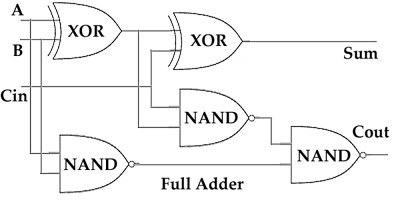
\includegraphics[width=.6\textwidth]{full_adder.png}
%\caption{A (claimed) full-adder circuit}
%\end{figure}

%\newcounter{rubricCat}
%\newcounter{rubricVal}
%\newlength{\colwidth}

%\newenvironment{rubric}[1]{%
%	\setcounter{GradeCategories}{#1}
%	\begin{landscape}
%	\begin{table}[t]
%	\begin{center}
%	\begin{tabulary}{.8\textwidth}{ l | *{5}{c}}
%	 & Excellent & Good & Acceptable & Needs Work & Absentee \\
%	 \end{tabulary}
%	 \end{center}
%	 \end{table}
%	\end{landscape}
%} % rubric environment

\end{document}
